%!TEX root = ../MasterThesis.tex

\section{A partially centralized \gls{P2P} system proposal}
\label{sec:p2p_partially_centralized_system}

In the \gls{E-commerce} fraud scenario, which has been selected for this Master thesis in Section~\ref{sec:scope_thesis}, the issuer of a credit card is the participant, who initiates a collaborative session to investigate the malicious online transactions. They are recognizing the active use (and maybe misuse) of a credit card in the online and the offline world first, and are also getting a notification about any suspicious activities from their fraud prevention systems. Due to these facts a valid design proposal for the \gls{E-commerce} fraud investigation system is based on the partially centralized \gls{P2P} architecture, in which the issuer of a credit card is taking over a leading position.

\subsection{Role of the issuer}
\label{subsec:p2p_partially_issuer_collecting}

In case a suspicious activity has been detected by the fraud prevention system of an issuer, one of the investigators from the issuer will initiate a collaborative session with the relevant stakeholders based on the usage history of the credit card in question. To establish the \gls{P2P} communication session the investigator is creating a new \gls{WebRTC} session in the collaborative system, which has been implemented as a Web application. By doing so the investigator will receive a unique session ID that can be transmitted to merchants, \gls{PSP}s and \gls{LSP}s to be able to join in the \gls{WebRTC} session. As the investigator is just being aware of the \gls{PSP}s affected they can invite them directly due to the existing business relationship between both parties. Based on the given credit card information the \gls{PSP}s can relate each payment authorization request to an order of an online merchant by referring to the payment authorization token. So the \gls{PSP}s will know the merchants that have to be involved in this \gls{E-commerce} fraud investigation, and can hand over contact information to invite them. Each online merchant can do likewise with the \gls{LSP} that has been used to handle the delivery of an order via the tracking number. \\

As soon as the relevant merchants, \gls{PSP}s and \gls{LSP}s have joined the \gls{P2P} communication session they will start sharing their information with the issuer. The information exchanged have been prepared as \gls{RDF} data sets by internal \gls{ETL} processes, and has been made available to the support staff of each stakeholder. In this process of information sharing the \gls{RDF} data sets of each stakeholder are replicated to the issuer, who will do the mapping and linking into a combined \gls{RDF} data store locally (as described in Section~\ref{sec:working_semantic_data}). This combination of the dispersed \gls{RDF} data sets will take place in a \gls{RDF} data store that the issuers have to setup and operate within their organization. Parts of this \gls{RDF} data store will take care of the reasoning over the merged \gls{RDF} data set to infer additional triple statements, as well as provide an internal \gls{SPARQL} endpoint to query the data store from the Web application as shown in Figure~\ref{fig:images_semweb_app}. \\

So the major tasks will be done on the side of the issuers, who are coordinating and executing the \gls{E-commerce} fraud investigations as depicted in Figure~\ref{fig:images_p2p_centralized}.\@

\begin{figure}[H]
	\centering
		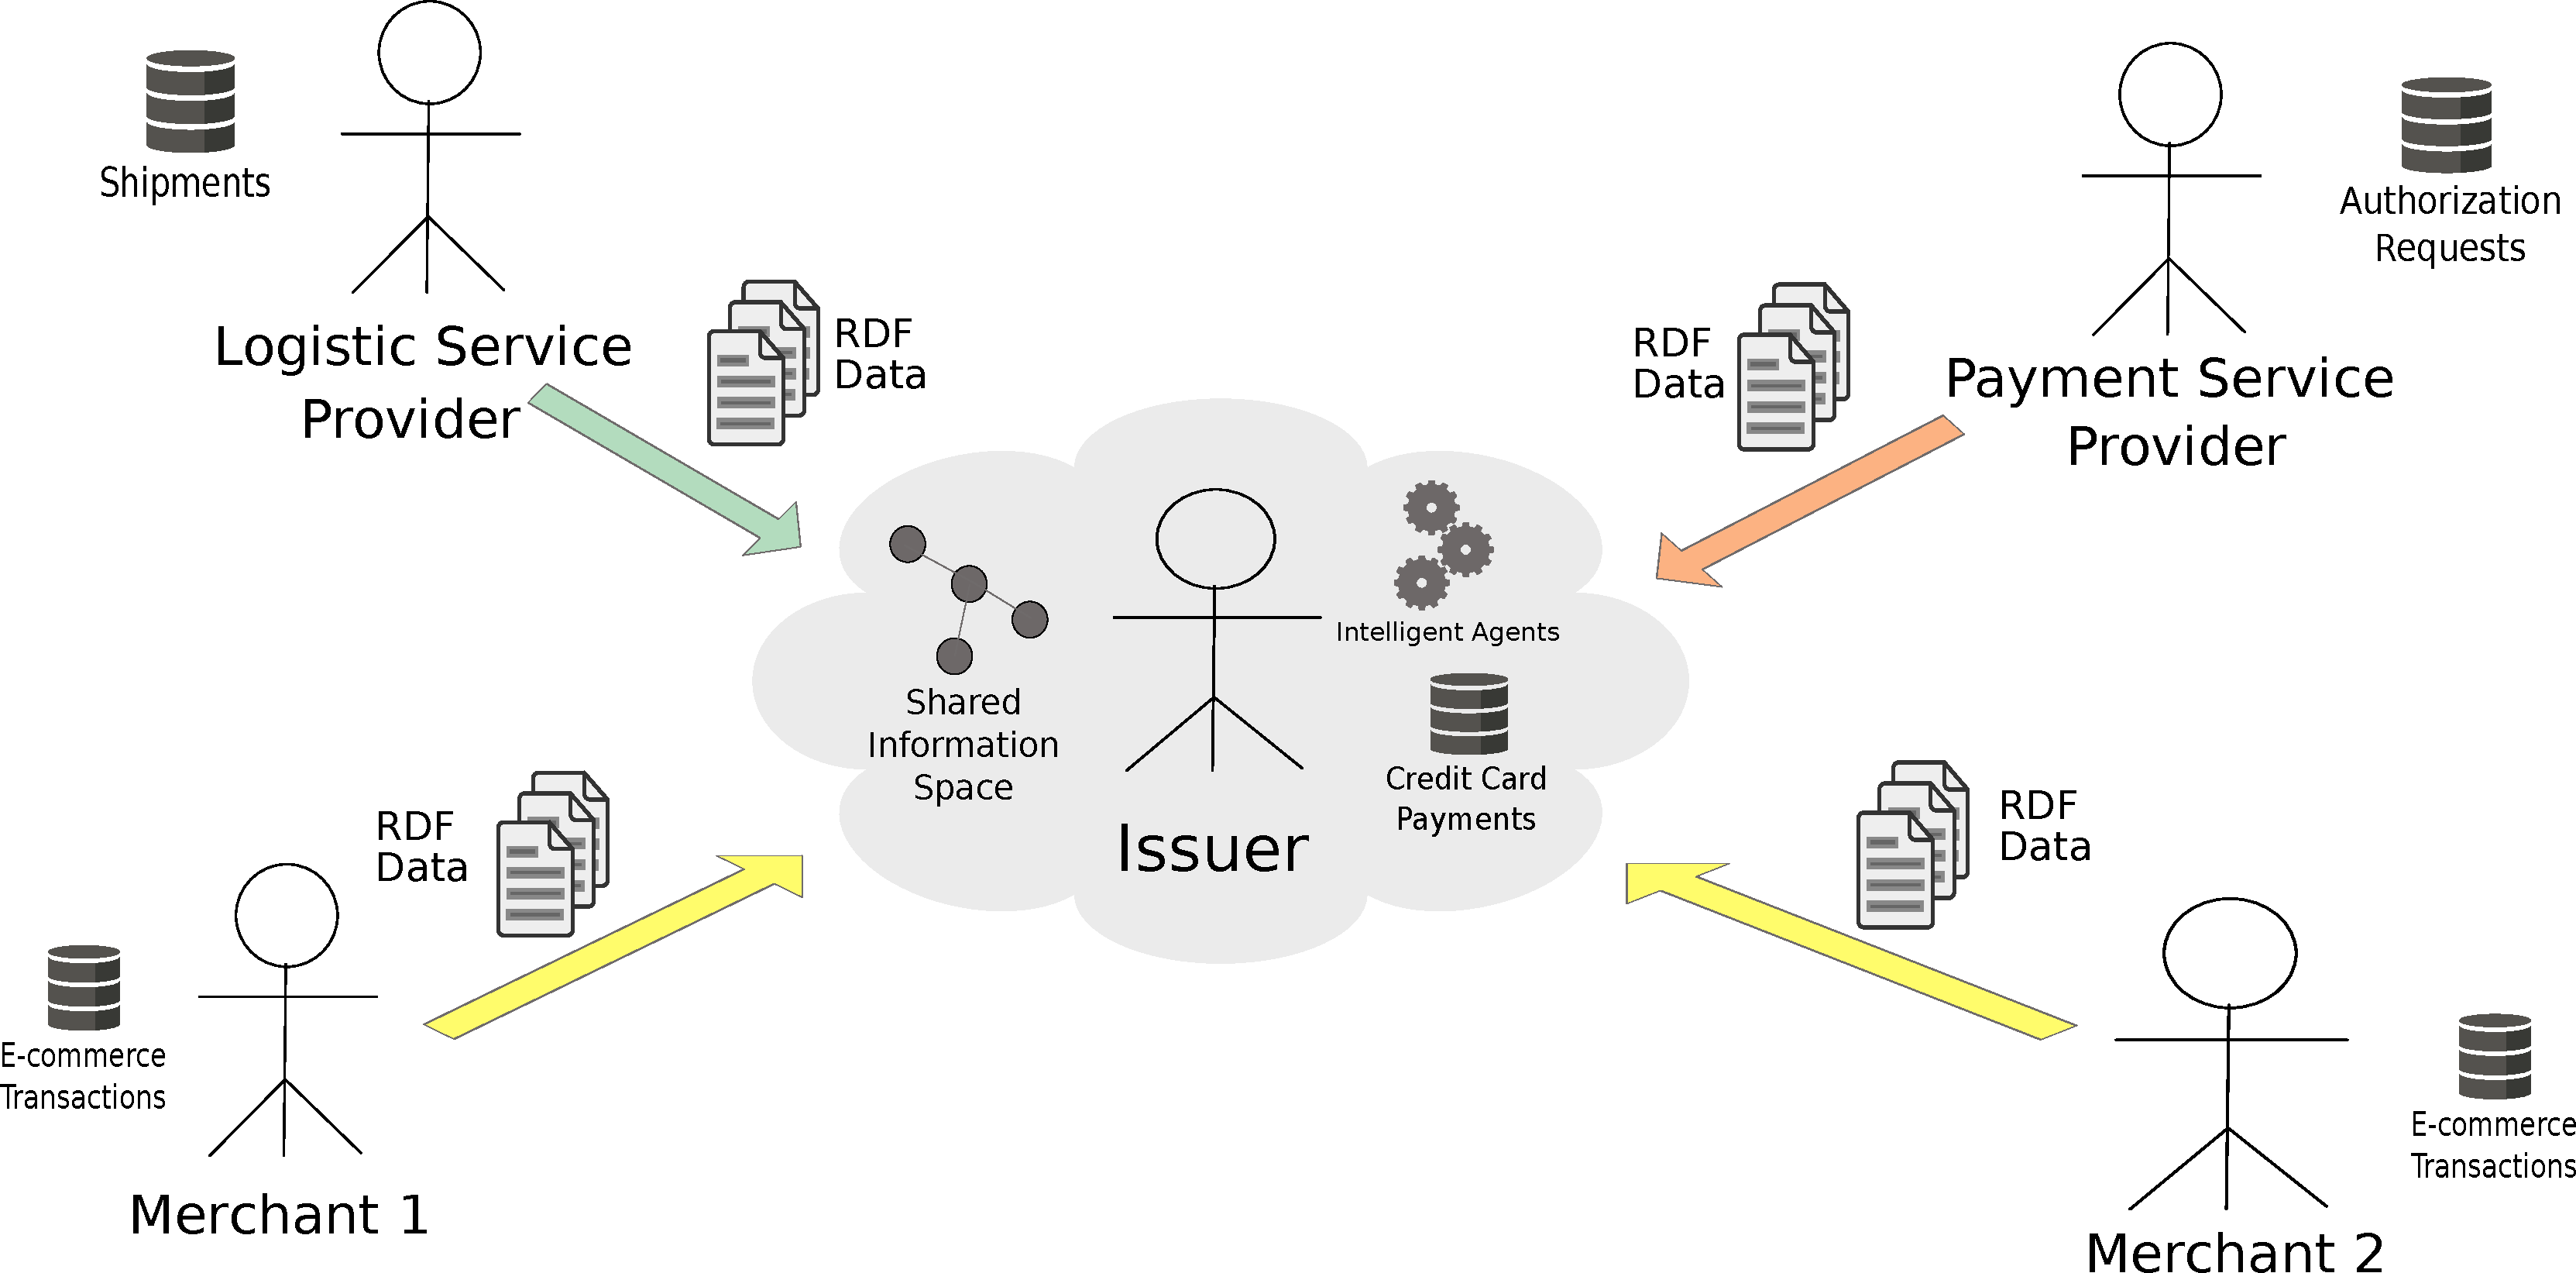
\includegraphics[width=0.9\columnwidth]{images/system_P2P_centralized.pdf}
	\caption{Collaborative system using a partially centralized \gls{P2P} architecture}
\label{fig:images_p2p_centralized}
\end{figure}


\subsection{Handling of privacy issues}
\label{subsec:p2p_partially_issuer_privacy}

One of the major concerns with the system architecture mentioned above is that the merchants, \gls{PSP}s and \gls{LSP}s have to hand over all of their relevant information to the issuer of a credit card for analyzing the \gls{E-commerce} activities. This can raise severe privacy issues as an issuer will receive a lot of detailed order information from the other parties within this collaborative system. Issuers can not only use these information for validating the correctness of malicious online transactions, but can also misuse them to build elaborate consumer profiles, which directly influence the scoring of that consumer in the internal credit and risk rating systems of the issuers. \\

In addition to that online merchants will likely not provide to much detail information about their sales and offerings in such a collaborative system, because of direct competitors might also be involved in the \gls{E-commerce} fraud investigation. By sharing parts of the business relevant information the merchants will fear that their internal business processes, pricing structures as well as customer loyalty activities get visible to their competitors and might lead to a stronger competition afterwards. \\



% subsec p2p_partially_centralized_system

% section design_proposal (end)
